\chapter{Flow Analysis}
\label{ch:flow_analysis}

Having evaluated individual software vulnerability patterns (such as \gls{sql} injection, \gls{xss}, memory overflows, and request forgery), it becomes essential to establish systematic mechanisms for discovering these weaknesses within real-world systems. Modern software scale and architectural complexity have expanded dramatically—spanning tens of millions to billions of lines of code (\gls{loc})—making manual code auditing unfeasible and positioning automated analysis as a fundamental requirement for secure system engineering.

\section{Verification vs. Validation}

Assuring system reliability and security requires two distinct quality control activities:

\begin{definition}{Verification vs. Validation}{verif-valid}
    \textbf{Verification} checks the internal consistency and compliance of an implementation against a specified model or requirement (answering: \textit{``Are you building it right?''}). \\
    \textbf{Validation} evaluates whether the final software product meets actual customer expectations and operational requirements (answering: \textit{``Are you building the right thing?''}).
\end{definition}

As illustrated across the development lifecycle, verification operates at unit, subsystem, and integration phases (via code reviews, static inspection, and unit/integration testing). Validation operates at the top level via acceptance testing, alpha/beta testing, and user trials.

\section{Static Analysis vs. Dynamic Analysis}

Software security analysis is fundamentally partitioned into two execution paradigms:

\begin{itemize}
    \item \textbf{Dynamic Analysis (Software Testing):} Involves executing the compiled target program with concrete test inputs and observing its runtime execution behavior, outputs, and system interactions.
    \item \textbf{Static Analysis (Software Inspection):} Involves analyzing static software artifacts (source code, intermediate representations, or configuration files) without executing the code directly.
\end{itemize}

\subsection{Dynamic Analysis Mechanics}
Dynamic testing requires generating concrete test cases to exercise system execution paths. Evaluating whether a test execution passes or fails requires a \textbf{test oracle}—a mechanism or specification defining the expected software behavior.

\begin{itemize}
    \item \textbf{Scope:} Testing checks only a finite subset of total software execution paths.
    \item \textbf{Defect Detection:} Dynamic execution can prove the \textit{presence} of bugs, but it can never prove their \textit{absence}.
    \item \textbf{Inaccuracy Classification:} Dynamic analysis is \textit{optimistically inaccurate}—because it cannot achieve exhaustive path coverage in non-trivial systems, passing test suites may lead to the false acceptance of faulty or vulnerable software.
\end{itemize}

\subsection{Static Analysis Mechanics}
Static analysis analyzes programs against pre-defined or fixed properties (such as prevention of null-pointer dereferences, memory buffer overruns, unvalidated input flows, resource leaks, or race conditions).

\begin{figure}[htpb]
\centering
\begin{tikzpicture}[node distance=1.8cm, auto, >=stealth, font=\small]
    % Dynamic Testing Path
    \node [draw, rectangle, fill=green!10, rounded corners, minimum width=3.2cm, minimum height=1.0cm, align=center] (dynamic) {\textbf{Dynamic Analysis}\\(Software Testing)};
    \node [draw, circle, fill=green!60!black, text=white, right=2.8cm of dynamic] (dyn-pass) {\checkmark};
    \node [draw, circle, fill=red!70!black, text=white, below=0.5cm of dyn-pass] (dyn-fail) {$\mathbf{X}$};
    
    \draw [->, thick] (dynamic) -- (dyn-pass) node[midway, above, font=\scriptsize] {Path Executed};
    \draw [->, thick] (dynamic) |- (dyn-fail) node[midway, below, font=\scriptsize] {Bug Triggered};
    \node [right=0.2cm of dyn-fail, font=\scriptsize] {Generates Input Case};

    % Static Analysis Path
    \node [draw, rectangle, fill=blue!10, rounded corners, minimum width=3.2cm, minimum height=1.0cm, align=center, below=2.0cm of dynamic] (static) {\textbf{Static Analysis}\\(Code Verification)};
    \node [draw, circle, fill=green!60!black, text=white, right=2.8cm of static] (stat-pass) {\checkmark};
    \node [draw, circle, fill=red!70!black, text=white, below=0.5cm of stat-pass] (stat-fail) {$\mathbf{X}$};
    
    \draw [->, thick] (static) -- (stat-pass) node[midway, above, font=\scriptsize] {All Paths Proved};
    \draw [->, thick] (static) |- (stat-fail) node[midway, below, font=\scriptsize] {Property Violated};
    \node [right=0.2cm of stat-fail, font=\scriptsize] {Generates Counterexample Trace};
\end{tikzpicture}
\caption{Operational comparison between dynamic execution testing and static verification.}
\label{fig:static-vs-dynamic-flow}
\end{figure}

\begin{itemize}
    \item \textbf{Path Exploration:} Static tools evaluate all program paths concurrently by constructing abstract representations.
    \item \textbf{Proving Properties:} Static analysis can establish safety properties across all possible executions (e.g., proving that a divide-by-zero exception is impossible).
    \item \textbf{Inaccuracy Classification:} Static analysis is \textit{pessimistically inaccurate}—because it operates over simplified abstract representations, it may report violations for safe execution paths, leading to the rejection of correct programs.
\end{itemize}

\section{Approximation and Alarm Classification}

According to Rice's Theorem\footnote{Check out ``CCC notes'' on github, section 2.4}, any non-trivial semantic property of a program is mathematically undecidable. Consequently, static analysis engines cannot compute exact reachable system states for complex codebases and must rely on abstract domains (e.g., mapping concrete integer values $\{0, 1, 2, 3, \dots\}$ to abstract properties such as $\text{even}$ or $\text{odd}$).

\subsection{Alarm Matrix}
When a static tool evaluates a security property, the output falls into one of four potential state classifications:

\begin{itemize}
    \item \textbf{True Positive (\gls{tp}):} An alarm is generated, and a genuine security vulnerability exists in the code.
    \item \textbf{False Positive (\gls{fp}):} An alarm is generated, but no actual vulnerability exists in the program (a false alarm).
    \item \textbf{False Negative (\gls{fn}):} No alarm is generated, but a real security vulnerability exists in the code (a missed vulnerability).
    \item \textbf{True Negative (\gls{tn}):} No alarm is generated, and the program is genuinely secure regarding that property.
\end{itemize}

\begin{figure}[htpb]
\centering
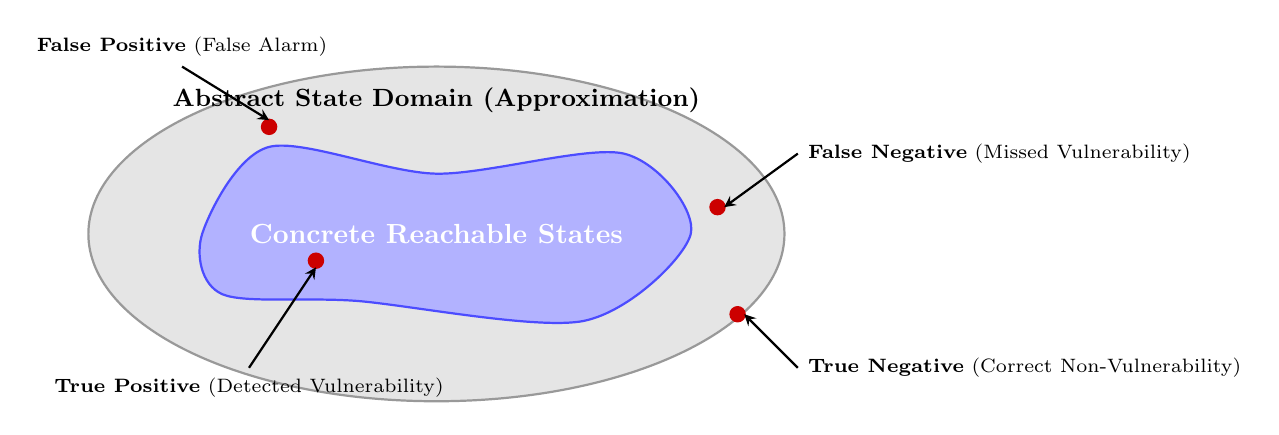
\begin{tikzpicture}[scale=0.85, >=stealth]
    % Outer Abstract State Space (Approximation)
    \draw[fill=gray!20, draw=gray!80, thick] (0,0) ellipse (5.2cm and 2.5cm);
    \node at (0, 2.0) {\small \textbf{Abstract State Domain (Approximation)}};
    
    % Inner Concrete Reachable States
    \draw[fill=blue!30, draw=blue!70, thick, smooth cycle] 
        plot coordinates {(-3.5,0) (-2.5,1.3) (0,0.9) (2.8,1.2) (3.8,0) (2.2,-1.3) (-1.2,-1.0) (-3.2,-0.9)};
    \node at (0, 0) {\color{white}\textbf{Concrete Reachable States}};
    
    % True Positive Point (Inside both)
    \fill[red!80!black] (-1.8, -0.4) circle (3.5pt);
    \draw[<-, thick] (-1.8, -0.5) -- (-2.8, -2.0) node[below, font=\scriptsize] {\textbf{True Positive} (Detected Vulnerability)};
    
    % False Positive Point (Inside approximation, outside concrete)
    \fill[red!80!black] (-2.5, 1.6) circle (3.5pt);
    \draw[<-, thick] (-2.5, 1.7) -- (-3.8, 2.5) node[above, font=\scriptsize] {\textbf{False Positive} (False Alarm)};
    
    % False Negative Point (Outside approximation, inside concrete - under-approximation scenario)
    \fill[red!80!black] (4.2, 0.4) circle (3.5pt);
    \draw[<-, thick] (4.3, 0.4) -- (5.4, 1.2) node[right, font=\scriptsize] {\textbf{False Negative} (Missed Vulnerability)};
    
    % True Negative Point (Outside both)
    \fill[red!80!black] (4.5, -1.2) circle (3.5pt);
    \draw[<-, thick] (4.6, -1.2) -- (5.4, -2.0) node[right, font=\scriptsize] {\textbf{True Negative} (Correct Non-Vulnerability)};
\end{tikzpicture}
\caption{Abstract state space approximation and alarm classifications.}
\label{fig:static-approximation-alarms}
\end{figure}

\subsection{Soundness vs. Completeness}
The direction of state space approximation dictates the tool's error characteristics:

\begin{itemize}
    \item \textbf{Sound Approximation (Over-approximation):} Encloses all concrete reachable states within a larger abstract domain. If a property holds in the over-approximation, it strictly holds in the concrete system. Sound analysis guarantees zero false negatives (no real bugs missed), but can generate a high volume of false positives.
    \item \textbf{Complete Approximation (Under-approximation):} Restricts the abstract domain to a strict subset of known safe reachable states. Complete analysis guarantees zero false positives, but can introduce false negatives (missing actual security flaws).
\end{itemize}

Commercial flow analysis tools frequently employ unsound over-approximations, intentionally trading off theoretical soundness to reduce false positive alarm volume to manageable levels for engineering teams.

\section{Control-Flow and Program Models}
\label{sec:control_flow_models}

To reason about dynamic runtime behaviors statically, programs are modeled as directed graphs representing control and data relationships. 

\begin{definition}{Control-Flow Graph (\glsfmtshort{cfg})}{cfg-def}
A \textbf{Control-Flow Graph} is a 4-tuple $\gls{cfg} = (N, E, n_e, n_x)$ where:
\begin{itemize}
    \item $N$ is the set of nodes, representing executable statements or basic blocks.
    \item $E \subseteq N \times N$ is the set of directed control-flow edges, where $(n, m) \in E$ indicates that statement $m$ can immediately succeed $n$ in execution semantics.
    \item $n_e \in N$ is the unique entry node of the program.
    \item $n_x \in N$ is the unique exit node of the program.
\end{itemize}
\end{definition}

\subsection{Control-Flow Paths and Independent Paths}
A path through a \gls{cfg} is a sequence of connected nodes and edges from $n_e$ to $n_x$. When a program contains loops, the total number of execution paths becomes infinite. To bound path coverage analysis, we compute linearly independent paths (paths introducing at least one edge not previously traversed).

The number of linearly independent paths in a strongly connected graph can be calculated using McCabe's metric:
\begin{equation}
\text{Independent Paths} = |E| - |N| + 2 = \text{Decisions} + 1
\end{equation}

\subsection{Dominators and Post-Dominators}
Understanding path dependencies requires formalizing control dominance:

\begin{itemize}
    \item \textbf{Pre-dominance:} Node $M$ pre-dominates node $N$ ($M \text{ dom } N$) if every path from entry $n_e$ to $N$ must pass through $M$.
    \item \textbf{Post-dominance:} Node $M$ post-dominates node $N$ ($M \text{ pdom } N$) if every path from $N$ to exit $n_x$ must pass through $M$.
    \item \textbf{Immediate Dominator:} The unique node $M$ closest to $N$ that strictly dominates $N$.
\end{itemize}

\subsection{Control Dependence}
Control dependence identifies which decision points dictate whether a given statement executes.

\begin{definition}{Control Dependence}{control-dep-def}
A node $F$ is \textbf{control-dependent} on a conditional node $B$ if and only if:
\begin{enumerate}
    \item Node $B$ has at least two execution successors (representing a branch decision).
    \item There exists a path from $B$ to $F$ such that $F$ post-dominates every node on the path after $B$.
    \item Node $B$ is \textit{not} post-dominated by $F$ (i.e., execution of $F$ is evitable at $B$).
\end{enumerate}
\end{definition}

A Control Dependence Graph (\gls{cdg}) explicitly represents these control relationships as directed edges, decoupling statement execution conditions from basic sequential ordering.

\section{Data Dependence and Def-Use Analysis}
\label{sec:data_dependence}

While control flow dictates execution order, statement interaction occurs primarily through variable values.

\begin{definition}{Def-Use (\glsfmtshort{du}) Pair}{du-pair-def}
A \textbf{Definition-Use (\glsfmtshort{du}) Pair} $(d, u)$ associates a program statement $d$ where a variable $v$ is assigned a value (a definition) with a statement $u$ where the value of $v$ is read (a use), provided there exists a \textbf{definition-clear path} from $d$ to $u$.
\end{definition}

\begin{itemize}
    \item \textbf{Definition ($Gen$):} Occurs at variable initializations, assignments, parameter receipts, or function calls modifying memory.
    \item \textbf{Use ($Use$):} Occurs when a variable's value is extracted in expressions, branch conditions, parameter passing, or return statements.
    \item \textbf{Killing a Definition ($Kill$):} If an intervening node $e$ assigns a new value to variable $v$, definition $v_e$ \textit{kills} definition $v_d$, terminating the definition-clear path.
\end{itemize}

\begin{figure}[htpb]
\centering
\begin{tikzpicture}[node distance=1.4cm, auto, >=stealth, font=\small]
    \node [draw, rectangle, fill=blue!10, rounded corners] (d1) {$A: \text{def } x$};
    \node [draw, rectangle, fill=red!10, rounded corners, below=0.8cm of d1] (d2) {$B: x = y \quad (\text{kills } x_A, \text{ defs } x_B)$};
    \node [draw, rectangle, fill=green!10, rounded corners, below=0.8cm of d2] (u) {$C: y = f(x) \quad (\text{uses } x_B)$};

    \draw [->, thick] (d1) -- (d2);
    \draw [->, thick] (d2) -- (u);
    
    \draw [->, thick, red, dashed] (d1.east) to [out=0, in=0] node[right, font=\scriptsize] {Path Killed by $B$} (u.east);
    \draw [->, thick, green!50!black] (d2.west) to [out=180, in=180] node[left, font=\scriptsize] {Definition-Clear Path $(B, C)$} (u.west);
\end{tikzpicture}
\caption{Definition-clear path versus killing a definition.}
\label{fig:def-clear-kill}
\end{figure}

\subsection{Path Explosion Problem}
Searching every individual \gls{cfg} path to find all reaching definitions is computationally intractable. Even in acyclic control flow graphs containing nested decision diamonds, the number of paths grows exponentially ($2^k$ paths for $k$ decisions). Practical static analysis algorithms avoid explicit path enumeration by calculating global summaries at each node over all incoming paths.

\section{Data-Flow Analysis Framework}
\label{sec:df_framework}

The Data-Flow Analysis framework formalizes static program analysis by setting up system systems of equations across nodes.

\subsection{Transfer Functions and Join Rules}
At each basic block or node $n$, data-flow states are propagated forward or backward using two core functions:

\begin{equation}
In(n) = \bigcup_{m \in Pred(n)} Out(m) \quad \text{(JOIN Rule / Confluence Operator)}
\end{equation}
\begin{equation}
Out(n) = f_n(In(n)) = (In(n) \setminus Kill(n)) \cup Gen(n) \quad \text{(TRANSFER Function)}
\end{equation}

Where:
\begin{itemize}
    \item $Gen(n)$ represents new definitions introduced within block $n$.
    \item $Kill(n)$ represents prior definitions overwritten by new assignments in block $n$.
\end{itemize}

\subsection{Iterative Worklist Algorithm}
To compute the exact reaching definitions across loops, an iterative fixed-point algorithm is applied:

\begin{algorithm}[H]
\caption{Iterative Reaching Definitions Algorithm}
\label{alg:reaching_definitions}
\begin{algorithmic}[1]
\State $Out[\text{Entry}] \gets \emptyset$
\For{each node $B \neq \text{Entry}$}
    \State $Out[B] \gets \emptyset$
\EndFor
\While{changes to any $Out$ set occur}
    \For{each node $B \neq \text{Entry}$}
        \State $In[B] \gets \bigcup_{p \in \text{Pred}(B)} Out[p]$
        \State $Out[B] \gets (In[B] \setminus \text{Kill}[B]) \cup \text{Gen}[B]$
    \EndFor
\EndWhile
\end{algorithmic}
\end{algorithm}

\subsection{Worked Example: Euclid's \glsfmtshort{gcd} Algorithm}
Consider dynamic data flow tracking within Euclid's \gls{gcd} procedure:

\begin{lstlisting}[language=Java]
public int gcd(int x, int y) {
    int tmp;             // Block A: def x_A, y_A, tmp_A
    while (y != 0) {     // Block B: use y
        tmp = x % y;     // Block C: def tmp_C; use x, y
        x = y;           // Block D: def x_D; use y
        y = tmp;         // Block E: def y_E; use tmp
    }
    return x;            // Block F: use x
}
\end{lstlisting}

Tracing the data flow equations for block $B$ and $E$ yields:
\begin{align}
In(B) &= Out(A) \cup Out(E) = \{x_A, y_A, tmp_A\} \cup Out(E)\\
Out(E) &= (In(E) \setminus \{y_A\}) \cup \{y_E\}
\end{align}
Through fixed-point iteration (or loop unrolling), we find that the definition of $x$ reaching the return statement at block $F$ can originate either from initial parameter $x_A$ (if the loop does not execute) or from internal iteration assignment $x_D$.

\subsection{Precision and Theoretical Solutions}
Static data-flow algorithms compute approximations of ideal theoretical execution properties:

\begin{itemize}
    \item \textbf{Meet Over All Paths (\gls{mop}):} Combines transfer functions across all structurally valid paths $p \in P_n$:
    \begin{equation}
    MOP[n] = \bigwedge_{p \in P_n} f_p(\top)
    \end{equation}
    \item \textbf{Meet Over Valid Paths (\gls{mvp} / Call String):} Restricts evaluation to valid interprocedural paths $VP_n$ matching call-return stack semantics.
    \item \textbf{Exact Solution ($EX$):} Restricts evaluation strictly to feasible paths $feas(P_n)$. Computing $EX[n]$ is undecidable in the general case due to correlated conditional branch infeasibility.
\end{itemize}

\begin{figure}[htpb]
\centering
\begin{tikzpicture}[node distance=1.2cm, auto, >=stealth, font=\small]
    \node [draw, rectangle, fill=gray!10] (b1) {1: \texttt{if (cond)}};
    \node [draw, rectangle, fill=blue!10, below left=0.6cm and 0.8cm of b1] (b3) {3: $x = \dots$};
    \node [draw, rectangle, fill=gray!10, below right=0.6cm and 0.8cm of b1] (b2) {2: $\dots$};
    \node [draw, rectangle, fill=gray!10, below right=0.6cm and 0.2cm of b3] (b4) {4: $\dots$};
    \node [draw, rectangle, fill=gray!10, below=0.6cm of b4] (b5) {5: \texttt{if (cond)}};
    \node [draw, rectangle, fill=red!10, below left=0.6cm and 0.8cm of b5] (b6) {6: $y = x + \dots$};

    \draw [->, thick] (b1) -- node[left, font=\tiny] {True} (b3);
    \draw [->, thick] (b1) -- node[right, font=\tiny] {False} (b2);
    \draw [->, thick] (b3) -- (b4);
    \draw [->, thick] (b2) -- (b4);
    \draw [->, thick] (b4) -- (b5);
    \draw [->, thick] (b5) -- node[left, font=\tiny] {False} (b6);

    \draw [->, ultra thick, red, dashed] (b1.north east) to [out=0, in=0] (b3.east) -- (b4.east) -- (b5.east) -- (b6.east);
\end{tikzpicture}
\caption{Path infeasibility caused by correlated branch conditions. Path $(3, 6)$ is reported by static flow graph analysis but cannot execute at runtime if \texttt{cond} remains unchanged.}
\label{fig:path-infeasibility}
\end{figure}

\subsection{Sensitivity and Analysis Scope}
The precision and computational complexity of data-flow analysis are determined by two main axes:

\begin{itemize}
    \item \textbf{Procedural Scope:} Intraprocedural analysis operates within a single procedure ($O(n^3)$ complexity). Interprocedural analysis operates across the entire global call graph.
    \item \textbf{Context Sensitivity:} Distinguishes procedure calls based on specific calling contexts (e.g., keeping analysis of function \texttt{sub()} separate when invoked from \texttt{foo()} versus \texttt{bar()}). Context-insensitive analysis merges call sites, introducing spurious return paths.
    \item \textbf{Flow Sensitivity:} Accounts for statement execution order. Flow-insensitive analysis ignores statement ordering, treating variables as global sets of values (useful for fast type checking, but imprecise for data tracking).
\end{itemize}

\subsection{Standard Data-Flow Security Applications}
Data-flow analysis forms the core foundation for several security and optimization passes:
\begin{itemize}
    \item \textbf{Taint Analysis:} Tracks untrusted user input (sources) along definition-clear paths to sensitive execution parameters (sinks, such as raw \gls{sql} queries or system commands).
    \item \textbf{Live Variable Analysis:} Determines whether a variable's value will be read downstream, identifying dead code or uninitialized memory reads.
    \item \textbf{Memory Safety Verification:} Detects memory release violations, such as double-free flaws or use-after-free pointer accesses.
\end{itemize}

\section{Data-Flow Structural Testing}
\label{sec:df_testing}

Data-flow information also provides rigorous structural criteria for dynamic software testing, bridging node/edge coverage and exhaustive path testing.

\begin{itemize}
    \item \textbf{All-Definitions Criterion:} Requires at least one test case to exercise a \gls{du} pair for every defined variable.
    \item \textbf{All-\glsfmtshort{du}-Pairs Criterion:} Requires at least one test case to exercise every reachable \gls{du} pair in the program.
    \item \textbf{All-\glsfmtshort{du}-Paths Criterion:} Requires test cases to exercise all simple (non-looping) definition-clear paths between every definition and use.
\end{itemize}

\section{Categories of Static Analysis}

Static analysis techniques are grouped into three core methodology layers:

\subsection{Pattern-Based Static Analysis}
Pattern-based analysis checks source code against predefined structural templates, syntactic rules, and industry coding policies (e.g., \gls{misra} guidelines for \textsf{C/C++}). It scans for syntactic code smells, deprecated function calls (such as \texttt{gets()} or \texttt{strcpy()}), and dangerous constructs. Rules can be customized by security teams to catch application-specific bug templates.

\subsection{Flow-Based Static Analysis}
Flow-based analysis models the logical execution paths of a program to track data value propagation and evaluate runtime interactions without code execution. It simulates value flows across functions, modules, and files, mapping source inputs (sources) to sensitive execution points (sinks) to expose vulnerabilities like \gls{sql} injection and taint propagation.

\subsection{Model Checking and Linear Temporal Logic}
Model checking performs an exhaustive state-space search over a finite-state model $M$ representing system behavior to verify whether a given temporal property $f$ holds ($M, s \models f$). Behavioral assertions are specified using \gls{ltl}.

\gls{ltl} extends standard propositional logic with temporal operators evaluated over execution sequences:
\begin{itemize}
    \item $\mathbf{X} \, p$ (\textbf{Next}): $p$ holds true in the immediate next state.
    \item $p \,\mathbf{U}\, q$ (\textbf{Until}): $p$ holds true continuously until $q$ becomes true.
    \item $\mathbf{F} \, p$ (\textbf{Finally}): $p$ holds true at some state in the future.
    \item $\mathbf{G} \, p$ (\textbf{Globally}): $p$ holds true continuously across all future states.
\end{itemize}

\subsubsection*{Example: State Model Verification}
Consider a microwave control state machine evaluated against safety properties:

\begin{itemize}
    \item $\mathbf{G}(\text{Heat} \rightarrow \text{Close})$: \textit{True.} Heating implies the door is closed.
    \item $\mathbf{G}(\text{Start} \rightarrow \mathbf{F} \, \text{Heat})$: \textit{False.} Stalling or error states can prevent heating.
    \item $\mathbf{G}((\text{Start} \land \neg\text{Error}) \rightarrow \mathbf{F} \, \text{Heat})$: \textit{True.} An error-free start guarantees eventual heating.
\end{itemize}

When an \gls{ltl} property evaluates to \textit{False}, the model checker generates an explicit counterexample path demonstrating the exact sequence of transitions that violates the property, providing an automated execution trace for debugging.